\documentclass{emulateapj}
\submitted{{\it Submitted for publication in ApJ}}
\usepackage{multirow,color,wrapfig,ulem}
\usepackage {graphicx}
\usepackage{graphics}
\usepackage[dvips]{epsfig}

%=========================================================================
%		INTERNAL MACROS
%=========================================================================
\def\be{\begin{equation}}
\def\ee{\end{equation}}
\def\ba{\begin{eqnarray}}
\def\ea{\end{eqnarray}}

% To highlight comments 
\definecolor{red}{rgb}{1,0.0,0.0}
\newcommand{\red}{\color{red}}
\definecolor{darkgreen}{rgb}{0.0,0.5,0.0}
\newcommand{\SRK}[1]{\textcolor{darkgreen}{\bf SRK: \textit{#1}}}
\newcommand{\SRKED}[1]{\textcolor{darkgreen}{\bf #1}}
\newcommand{\before}[1]{\textcolor{red}{ #1}}
\newcommand{\after}[1]{\textcolor{darkgreen}{ #1}}

\newcommand{\LCDM}{$\Lambda$CDM~}
\newcommand{\beq}{\begin{eqnarray}}  
\newcommand{\eeq}{\end{eqnarray}}  
\newcommand{\zz}{$z\sim 3$} 
\newcommand{\avg}[1]{\langle{#1}\rangle}  
\newcommand{\ly}{{\ifmmode{{\rm Ly}\alpha}\else{Ly$\alpha$}\fi}}
\newcommand{\hMpc}{{\ifmmode{h^{-1}{\rm Mpc}}\else{$h^{-1}$Mpc}\fi}}  
\newcommand{\hGpc}{{\ifmmode{h^{-1}{\rm Gpc}}\else{$h^{-1}$Gpc}\fi}}  
\newcommand{\hmpc}{{\ifmmode{h^{-1}{\rm Mpc}}\else{$h^{-1}$Mpc}\fi}}  
\newcommand{\hkpc}{{\ifmmode{h^{-1}{\rm kpc}}\else{$h^{-1}$kpc}\fi}}  
\newcommand{\hMsun}{{\ifmmode{h^{-1}{\rm {M_{\odot}}}}\else{$h^{-1}{\rm{M_{\odot}}}$}\fi}}  
\newcommand{\Mmin}{{\ifmmode{{M_{\rm min}}}\else{${M_{\rm min}}$}\fi}}
\newcommand{\mmin}{{\ifmmode{{M_{\rm min}}}\else{${M_{\rm min}}$}\fi}}
\newcommand{\mmax}{{\ifmmode{{M_{\rm max}}}\else{${M_{\rm max}}$}\fi}}
\newcommand{\lmmin}{{\ifmmode{{\log M_{\rm min}}}\else{${\log M_{\rm min}}$}\fi}}
\newcommand{\lmmax}{{\ifmmode{{\log M_{\rm max}}}\else{${\log M_{\rm max}}$}\fi}}

\newcommand{\Mmax}{{\ifmmode{{M_{\rm max}}}\else{${M_{\rm max}}$}\fi}}
\newcommand{\dm}{{\ifmmode{{\Delta M}}\else{$\Delta M$}\fi}}
\newcommand{\dlm}{{\ifmmode{{\Delta \log M}}\else{$\Delta \log M$}\fi}}
\newcommand{\focc}{{\ifmmode{{f_{\rm occ}}}\else{${f_{\rm occ}}$}\fi}}

\newcommand{\Msun}{{\ifmmode{{\rm {M_{\odot}}}}\else{${\rm{M_{\odot}}}$}\fi}}  
\newcommand{\msun}{{\ifmmode{{\rm {M_{\odot}}}}\else{${\rm{M_{\odot}}}$}\fi}}  
\newcommand{\lya}{{Lyman$\alpha$~}}
\newcommand{\clara}{{\texttt{CLARA}}~}
\newcommand{\rand}{{\ifmmode{{\mathcal{R}}}\else{${\mathcal{R}}$ }\fi}}  
%SAMPLES


%MY COMMANDS #############################################################
\newcommand{\sub}[1]{\mbox{\scriptsize{#1}}}
\newcommand{\dtot}[2]{ \frac{ d #1 }{d #2} }
\newcommand{\dpar}[2]{ \frac{ \partial #1 }{\partial #2} }
\newcommand{\pr}[1]{ \left( #1 \right) }
\newcommand{\corc}[1]{ \left[ #1 \right] }
\newcommand{\lla}[1]{ \left\{ #1 \right\} }
\newcommand{\bds}[1]{\boldsymbol{ #1 }}
\newcommand{\oiint}{\displaystyle\bigcirc\!\!\!\!\!\!\!\!\int\!\!\!\!\!\int}
\newcommand{\mathsize}[2]{\mbox{\fontsize{#1}{#1}\selectfont $#2$}}
\newcommand{\eq}[2]{\begin{equation} \label{eq:#1} #2 \end{equation}}
\newcommand{\lth}{$\lambda_{th}$ }
\newcommand{\reff}{{\ifmmode{r_{\mbox{\tiny eff}}}\else{$r_{\mbox{\tiny eff}}$}\fi}}
%#########################################################################

%TO DO COMMANDS. Highlight region that needs extra work  #############################################################
\newcommand{\todo}{\ifmmode \text{\Huge{\(\bullet\)}} \else {\Huge$\bullet$}\fi}
% \newcommand{\todo}{\ifmmode {\Huge \bullet} \else {\Huge$\bullet$}\fi}
\newcommand{\tido}{\ifmmode {\bullet} \else $\bullet$\fi}
\newcommand{\REFS}{(\todo REFS) }
\newcommand{\toref}{(\todo REFS)}
%#########################################################################



\begin{document}
%=========================================================================
%		FRONT MATTER
%=========================================================================
\title{Uncertainty on the galaxy-halo connection for Lyman-$\alpha$ emitters at $z=3.1$}
\author{
  Juli\'an E. Mej\'ia-Restrepo \thanks{jemejia@das.uchile.cl}$^{1,3}$,
  Jaime E. Forero-Romero \thanks{je.forero@uniandes.edu.co}$^{2}$ 
}

\affil{
$^1$Departamento de Astronom\'{i}a, Universidad de Chile, Camino el Observatorio 1515, Santiago, Chile\\
$^2$Departamento de F\'{i}sica, Universidad de los Andes, Cra. 1
No. 18A-10, Edificio Ip, Bogot\'a, Colombia\\
$^3$FACom-Instituto de F\'isica-FCEN, Universidad de Antioquia, Calle 70 No. 52-21, Medell\'in, Colombia
}





\begin{abstract}
We study the impact of cosmic variance and observational uncertainties in constraining the mass and  occupation fraction ($f_{\rm occ}$) of dark matter halos hosting \ly\ Emitting  Galaxies at high redshift (LAEs).
We use a N-body simulation to construct mock catalogs with the same typical size  of observed fields at $z=3.1$ ($\sim 1 {\rm deg^2}$) to match the observed  angular correlation function (ACF) and number density of LAEs.  
In our model a dark matter halo with mass in the range $M_{\rm min}<M_{\mathrm h}<M_{\rm   max}$ can only host one detectable LAE at most. By following a thorough Markov Chain Monte-Carlo exploration of the parameter space determined by $M_{\rm min}$ and $M_{\rm   max}$, our analysis shows that $f_{\rm occ}$ is uniquely determined by $M_{\rm min}$ regardless of $M_{\rm max}$ using the relation $\focc\sim0.1\left(\mmin/10^{10.5}\right)^{0.93}$ . 
However, the current observational data only allows us to put weak constraints on $M_{\rm min}$, $M_{\rm max}$ and consequently on $f_{\rm occ}$. 
Particularly, we find that $10^{9.6}\hMsun\leq M_{\rm min}\leq 10^{11.0}\hMsun$ , $10^{10.9}\hMsun\leq M_{\rm max}\leq 10^{13.0}\hMsun$ and $0.02\leq f_{\rm occ}\leq 0.30$. 
Nevertheless, we also find that  the upcoming large surveys can help to put tighter constraints on $M_{\rm min}$ and $f_{\rm occ}$ through the width measurement of the LAE number distribution function obtained over several fields of the same size of current observations. 
Analogously, the  improvement in the precision of the measured ACF will assist in constraining $M_{\rm max}$.  
\end{abstract}

\keywords{
Cosmology: theory - large-scale structure of Universe -
Methods: data analysis - numerical - N-body simulations
}

% JF - 1. Intro 3/10
% JF - 2. Methodology 1/7

%*************************************************************************
\section{Introduction}
\label{sec:introduction}
\toref ADD NEWER REFERENCES
Lyman-$\alpha$ emitting galaxies (LAEs) are central to a wide range
of subjects in extragalactic astronomy. 
LAEs can be used as probes of reionization \citep{Dijkstra11}, tracers of large scale structure \citep{Koehler2007},  signposts for low metallicity stellar populations, markers of the galaxy formation process at high redshift \citep{Dayal2009,ForeroRomero2012} and tracers of active star formation \citep{Guaita2013}. 

In most of those cases, capitalizing the observations requires  understanding how LAEs are formed within an explicit cosmological context. 
Under the current structure formation paradigm the dominant matter content of the Universe is dark matter (DM). 
Each galaxy is thought to be hosted by a larger dark matter structure known as a halo. \citep{Peebles1980,SpringelNature05}. 
Understanding the cosmological context of LAEs thus implies studying the galaxy-halo connection. 
Galaxy formation models suggest that the physical processes that regulate the star formation cycle are dependent on halo mass \citep{Behroozi2013a}.
The mass becomes the most important element in the halo-galaxy connection. 
   
The goal becomes finding the typical DM halo mass of halos hosting LAEs.
In the case of LAEs there are different ways to find this mass range.
One approach is theoretical, using general astrophysical principles to find the relationship between halo mass, intrinsic \ly\ luminosities and observed \ly\ luminosities. This approach is usually implemented through semi-analytic models \citep{Garel2012,Orsi2012} and  full N-body hydrodynamical simulations \citep{Laursen2007, Dayal2009, ForeroRomero2011, Yajima2012}. 

%JF

The downside of these calculations is the uncertainty in the estimation of the escape fraction of \ly\ photons. Given the resonant nature of the \ly\ line, the escape fraction is sensitive to  the dust contents, density, temperature, topology and kinematics of the neutral Hydrogen in the interstellar medium (ISM). The process of finding a consensus on the expected value
for the \ly\ escape fraction in high redshift galaxies is still matter
of open debate
\citep{Neufeld1991,Verhamme2006,ForeroRomero2011,Dijkstra2012,Laursen2013,Orsi2012}.

A different approach to infer the typical mass of halos hosting
LAEs is based on the spatial clustering information. 
This approach uses the fact
that in CDM cosmologies the spatial clustering of galaxies on large
scales is entirely dictated by the halo distribution
\citep{Colberg00}, which in turn has a strong dependence on halo
mass. 
Using measurements of the angular correlation function of LAEs,
observers have put constraints on the typical mass and occupation
fraction of the putative halos hosting these galaxies
\citep{Hayashino2004,Gawiser07,Nilsson2007,Ouchi2010,Bielby16}. 
In these studies the observations are done on fields of $\sim 1$ deg$^{2}$ and
the conclusions derived on the halo host mass do not elaborate on the uncertainty resulting from the cosmic variance on these fields.

In this letter we investigate the impact of cosmic variance in
constraining the mass and occupation fraction of halos hosting LAEs at $z=3$.
We build mock surveys from a cosmological N-body to compare them against the observations in \cite{Bielby16} using the angular correlation function. 
We use a simple model to populate a halo in the simulation with a LAE   
assuming a minimum (\mmin) and maximum mass (\mmax) for the dark matter halos hosting LAEs without predicting a \ly\  luminosity. 
This approach bypasses all the physical uncertainties associated to star formation and radiative transfer.
We use the Markov Chain Monte Carlo technique to obtain the likelihood of the parameters given the observational constraints.

Throughout this letter we assume a $\Lambda$CDM cosmology with the
following values for the cosmological parameters, $\Omega_{m}=0.30711$,
$\Omega_{\Lambda}=0.69289$ and $h=0.70$, corresponding to the matter
density, vacuum density and the Hubble constant in units of 100 km
s$^{-1}$ Mpc$^{-1}$. 


\begin{figure}
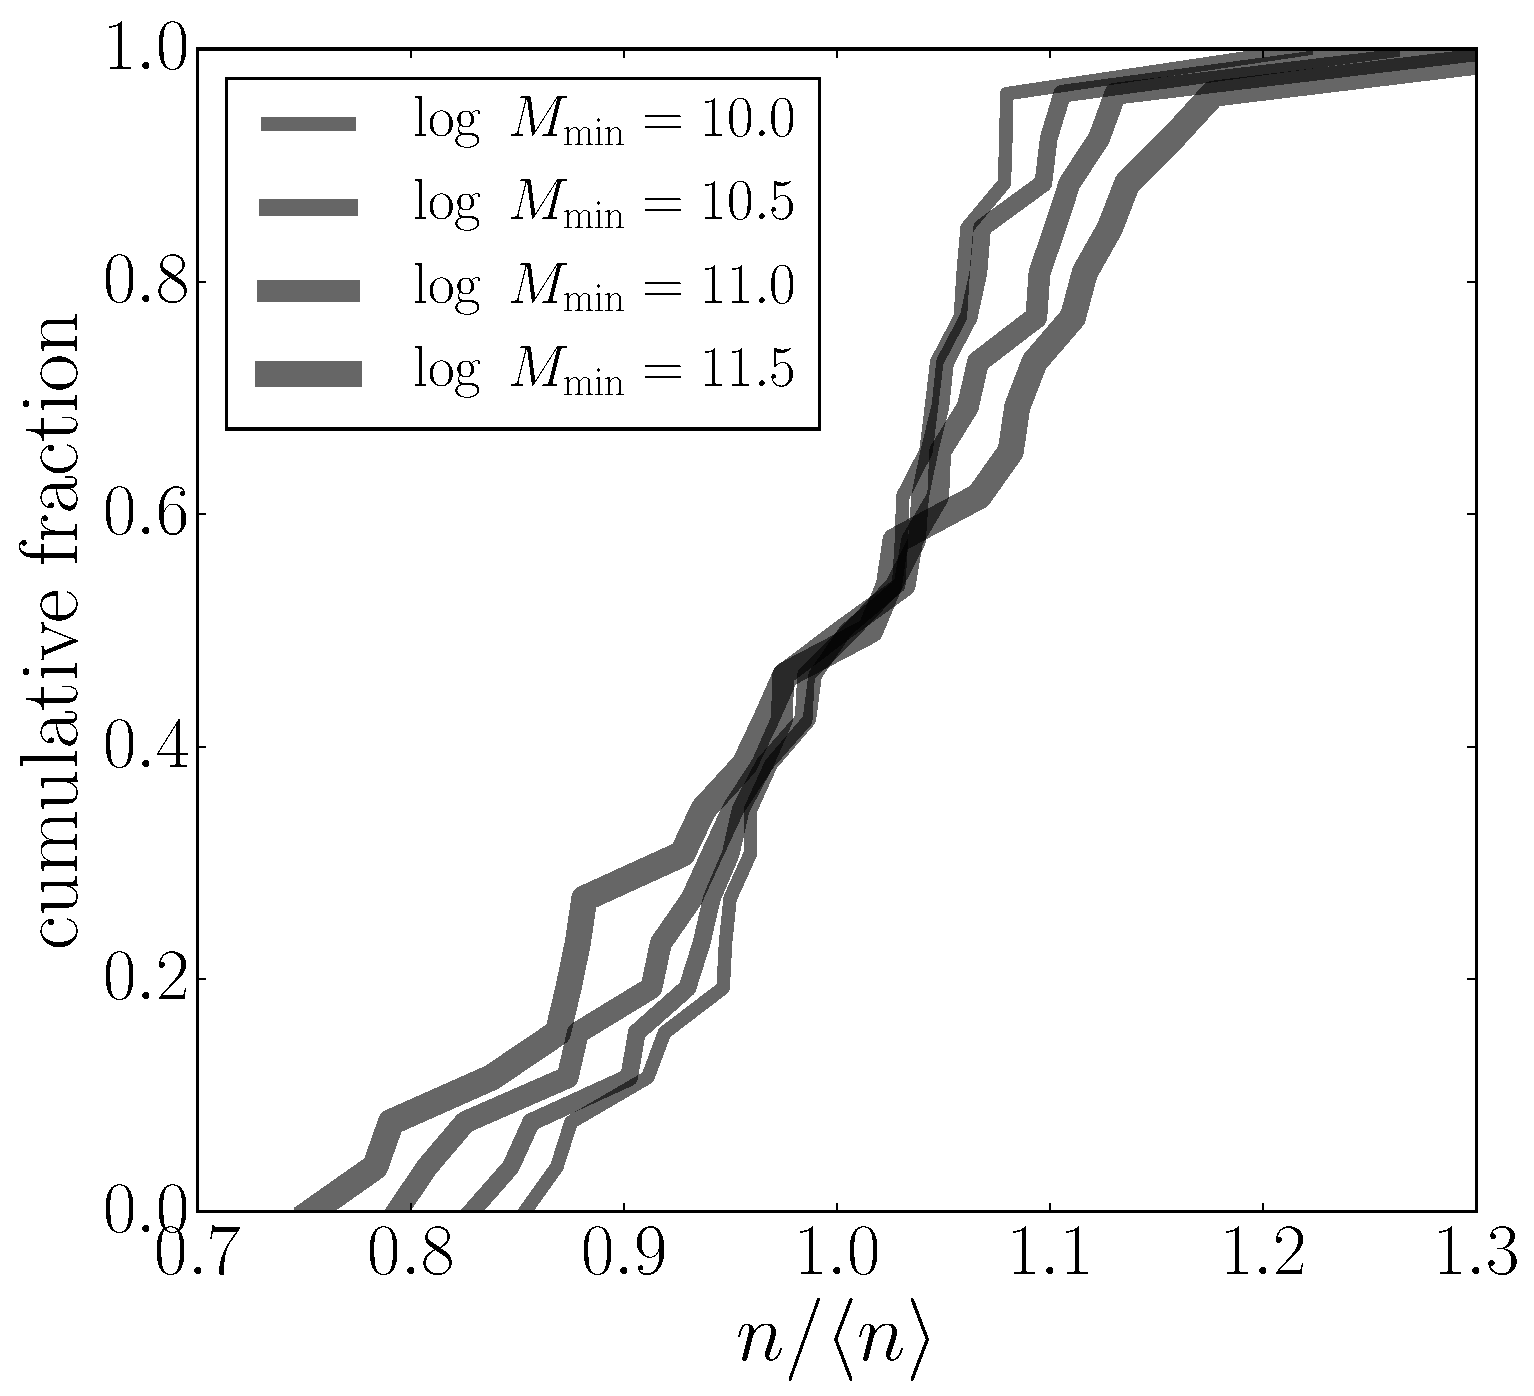
\includegraphics[width=0.47\textwidth]{fig1.pdf}
\caption{Cumulative halo number density distribution function over
  27 mock fields. Each line corresponds to a
  different model with increasig values of $M_{\rm min}$. 
  Different models produce different number density distributions. The
width increases with \mmin. } 
\label{fig:cosmicv0}
\end{figure}

\section{Methodology}

The base of our method is the comparison between observations and mock
catalogs. 
This approach allows us to take explicitly into account cosmic variance. 
The comparison has four key elements. First, the observations we take as a benchmark. Second, the N-body simulation and the halo catalogs we use to build the mocks. Third, the parameters describing our model to assign a LAE to a halo. Fourth, the statistical method we adopt to compare observations and simulations.
We describe in detail these four elements in the following subsections.


\begin{figure*}
\begin{center}
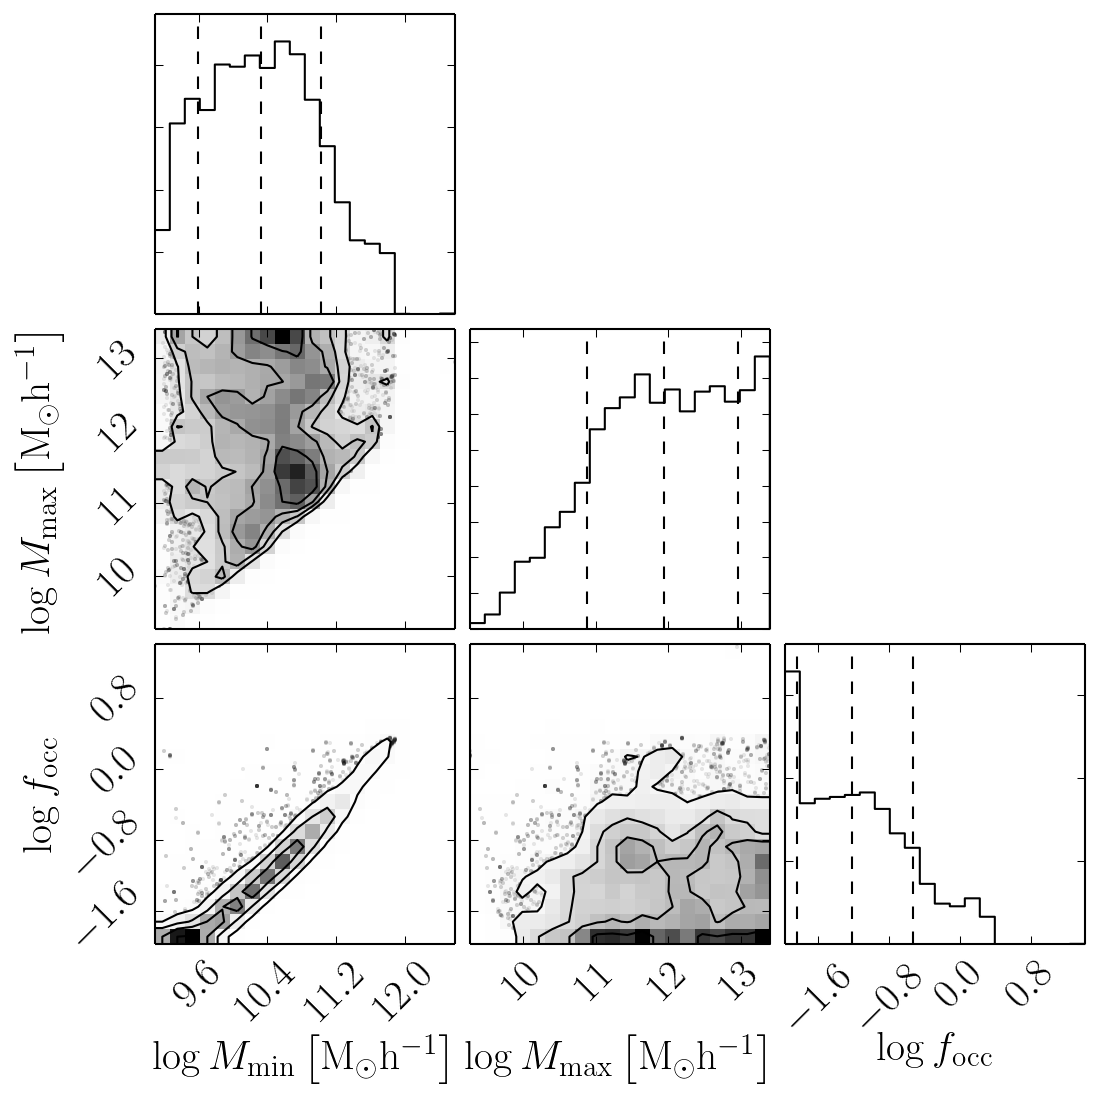
\includegraphics[width=0.85\textwidth]{likelyplot_1deg_total.png}
\end{center}
\caption{One and two dimensional projections of the posterior
  probability distributions of \mmin, \mmax\ and \focc\ as described in
  the label of each sub-figure. We remark that
those models where $\log \focc>0.00$ ($\focc>1$) correspond  to models where the number density  of halos is smaller than the number of observed LAEs but are
still consistent because of the uncertainty in the median number
density of LAEs in the universe due to cosmic variance. See
Fig. \ref{fig:cosmicv0} and \S\ref{subsec:explore} for details.} 
\label{fig:like}
\end{figure*}

\subsection{Observational constraints}
\label{subsec:obs}
\citet{Bielby16} used narrow band imaging to detect 643 LAE candidates
at $z\sim 3$  with equivalent widths of $\gtrsim$65\AA\ and a flux limit
of $2\times10^{17}{\rm erg/cm^2/s}$ ($L\sim 7\times10^{42}{\rm erg/s} $). 
Using spectroscopy they found a 22\% contamination fraction.
Their observations cover 5 (out of 9) independent and co-spatial fields of the VLT LBG Redshift Survey (VLRS). 
The  total observed  area corresponds to 1.07$\rm deg^2$ that translates to
$\sim$80$^2\hMpc^2$ in a comoving scale. \citet{Bielby16} used the
NB497  narrow-band filter whose 77\AA\ FWHM and 154\AA\ FWTM correspond to a total observational depth of 44\hMpc\  and 82\hMpc\ comoving, respectively.

%JF

\subsection{Simulation and halo catalog}
\label{subsec:sim}

We use results from the  Bolshoi simulation \citep{Bolshoi} which was performed in a cubic volume of 250 $h^{-1}$ Mpc comoving on a side. The dark matter distribution was sampled using  $2048^{3}$ particles. The cosmological parameters are consistent with Planck 2013 results \citep{Planck2014} with a matter density
$\Omega_{\rm m} = 0.307$, cosmological constant
$\Omega_{\Lambda}=0.693$, dimensionless Hubble constant $h=0.70$, slope
of the power spectrum  $n=0.96$ and normalization of the power
spectrum $\sigma_{8}=0.82$.  
This translates into a particle mass of  $m_{\rm p}=1.54\times 10^{8}$ $h^{-1}$ M$_{\odot}$.  

We use halo catalogs constructed with a Bound-Density-Maxima (BDM) algorithm. The catalogs were obtained from the publicly available
Multidark database  \footnote{{\tt
    http://www.multidark.org/MultiDark/}} \citep{MultiDark}. For each
halo in the box we extract its comoving position and mass. 
We focus our work on halos more massive than $1.54\times 10^{9}$\hMsun\ resolved with at least  $10$ particles.
%the reasons for this choice are explained in the next sub-section. 

We divide the total volume of the snapshot of the simulation at z$\sim$3
into  27 smaller mock volumes mimicking the  comoving area and depth  
reported in \citet{Bielby16} and described in \S \ref{subsec:obs}. 
This allows  us to take explicitly into account the effects of cosmic variance.

\subsection{A model to populate halos with LAEs}
\label{subsec:mocks}

We build a model to assign LAEs to a DM halo. 
We are not concerned on the exact LAE luminosity, we only care about a yes/no answer to the following question. Does this halo host a LAE?

We first assume that a dark matter halo can host one detectable LAE at most.  
This assumption is consistent with theoretical analysis of the correlation function \citep{Jose2013b} and observations that confirm a lack of class pairs in LAEs \cite{Bond2009}. 

Then we say that a halo will host a LAE with probability $f_{\rm occ}$ if and only if the halo mass is in the range $M_{\rm min}< M_{\mathrm h} < M_{\rm max}$.
The probability $f_{\rm occ}$ can be thought as the occupation fraction of halos which can be automatically set as the ration of the observed number of LAEs to the number of halos within the considered mass range, that is $f_{\rm occ}\equiv N_{\rm LAE}/N_{\mathrm halos}$.

Fig. \ref{fig:cosmicv0}  shows the cumulative halo number distribution (HND) in the  mock fields of the simulation for different models $\mathcal{M}$. From this figure we can see that the number of dark matter halos along the mock fields for different models $\mathcal{M}$ varies within a factor of $\sim 2$ ($\sim 0.3$dex) tracing the cosmic variance. As a consequence, the occupation fraction varies along  the mock fields  by the same factor factor. The interpretation of the occupation fraction $f_{\rm occ}$ involves two phenomena: the actual presence of a star forming galaxy in a halo and its detectability as a LAE. 

We do not explore any physical model to disentangle these two effects. This means that our model does not assign a luminosity or escape fraction to each
LAE.
We avoid this in order to maintain theoretical uncertainties to a minimum. 
This flexibility allows us to explore a wide range of possible masses for
the host halos without any strong theoretical prejudice regarding the
details of star formation and \ly\  escape fraction.

We also artificially contaminate our mock catalogs with 22$\%$ randomly distributed data points to mimic the fraction of interlopers in observations \citet{Bielby16} .
On top of that we apply rejection sampling  to our LAE selection taking the transmission function of the NB479 filter used in their observations as a radial selection factor.

In what follows we note by the letter ${\mathcal M}$ a model
defined by a particular choice of the two parameters $M_{\rm min}$, 
$M_{\rm  max}$. For each model  ${\mathcal M}$ we define $\tilde{f}_{\rm occ}$ as the median occupation fraction within the the mock fields and  $\Delta M \equiv \mmax-\mmin$.

\subsection{Exploring and selecting consistent models}
\label{subsec:explore}
We use the angular correlation function to compare the observations with our mock catalogs. 
This is done trough a thorough exploration of the parameter space of the models ${\mathcal M}$ by  means of a Monte Carlo Markov Chain minimization using  the EMCEE python package \citep{emcee2013}.
We put a flat prior on $\log M_{\rm min}$ and $\log \mmax$ to vary between $9.2$ up to $13.4$, corresponding to the halo mass range of the simulation at $z=3$. 
Given that the typical scatter  in $N_{\mathrm halos}$ is about 0.3 dex (i.e. about  a factor of 2), our parameter space is restricted to models where the median number of dark matter halos is larger than  $N_{\rm LAE}/3$. Because of this posibility of having $N_{\mathrm halos}$  smaller than $N_{\rm LAE}$ there will be some models where    $\focc\equiv N_{\rm LAE}/N_{\rm halo}>1$. Those models only reflect the uncertainty in the number density of LAEs due to cosmic variance.


The MCMC exploration is done using a total of 24 seeds and 400
iterations (9600 models) to sample the posterior PDF,  $P(\mmin,
\mmax, f_{\rm occ}| \mathcal{M}) \propto \exp(-\chi_{\mathcal
  M}^2/2)$, with 

\begin{equation}
\chi_{\mathcal M}^2=\sum_{\theta}\left[\frac{\left( \rm{ACF}_{\mathcal M}\left(\theta\right) - \rm{ACF}_{\rm obs}\left(\theta\right)\right)^2}{ \sigma_{\rm \mathcal M}^{2}\left(\theta\right) + \sigma_{\rm obs}^{2}\left(\theta\right)}\right]
\end{equation}
%
where  $\rm{ACF}_{\mathcal M}$ and  $\rm{ACF}_{\rm obs}$ are the ACF
of the explored model ${\mathcal M}$ and the observational ACF
reported by \citet{Bielby16} respectively. $\sigma_{\rm \mathcal M}$
is the associated 1-$\sigma$ scatter  of the $\rm{ACF}_{\mathcal M}$
as a product of cosmic variance and  $\sigma_{\rm obs}$ is the
observational error associated to $\rm{ACF}_{\rm obs}$.  The
$\rm{ACF}_{\mathcal M}$s are computed using the Landy \&  Szalay
estimator  \citep{Landy1993}.  




\section{Results and Discussion}




\subsection{Constraining \mmin, \mmax\ and \focc\ in Dark Matter Halos hosting LAEs} 

In Fig. \ref{fig:like} we present yhe one and two dimensional
projections of the posterior probability distributions of \mmin, \mmax
and \focc. We find that the \mmin and \mmax parameter space cannot be
tightly constrained mainly because of cosmic variance and the large
observational Poisonnian uncertainty in the ACF. We however found that
9.6$<\log \mmin<$11.0 and 10.9$<\log\mmax<$13.0.   We interestingly
find that \focc\ is basically completely determined by \mmin  going
from \focc$=$0.015 when $\log\mmin=$9.6 to \focc$=$0.30 when
$\log\mmin=$11.0
($\focc\sim0.1\left(\mmin/10^{10.5}\right)^{0.93}$). We remark that
those models where $\log \focc>0.00$ ($\focc>1$) correspond  to models where the number density  of halos is smaller than the number of observed LAEs but are
still consistent because of the uncertainty in the median number
density of LAEs in the universe due to cosmic variance (see
Fig. \ref{fig:cosmicv0} and \S\ref{subsec:explore}).%in the number of dark matter halos along the
                         %mock fields  

\begin{figure}
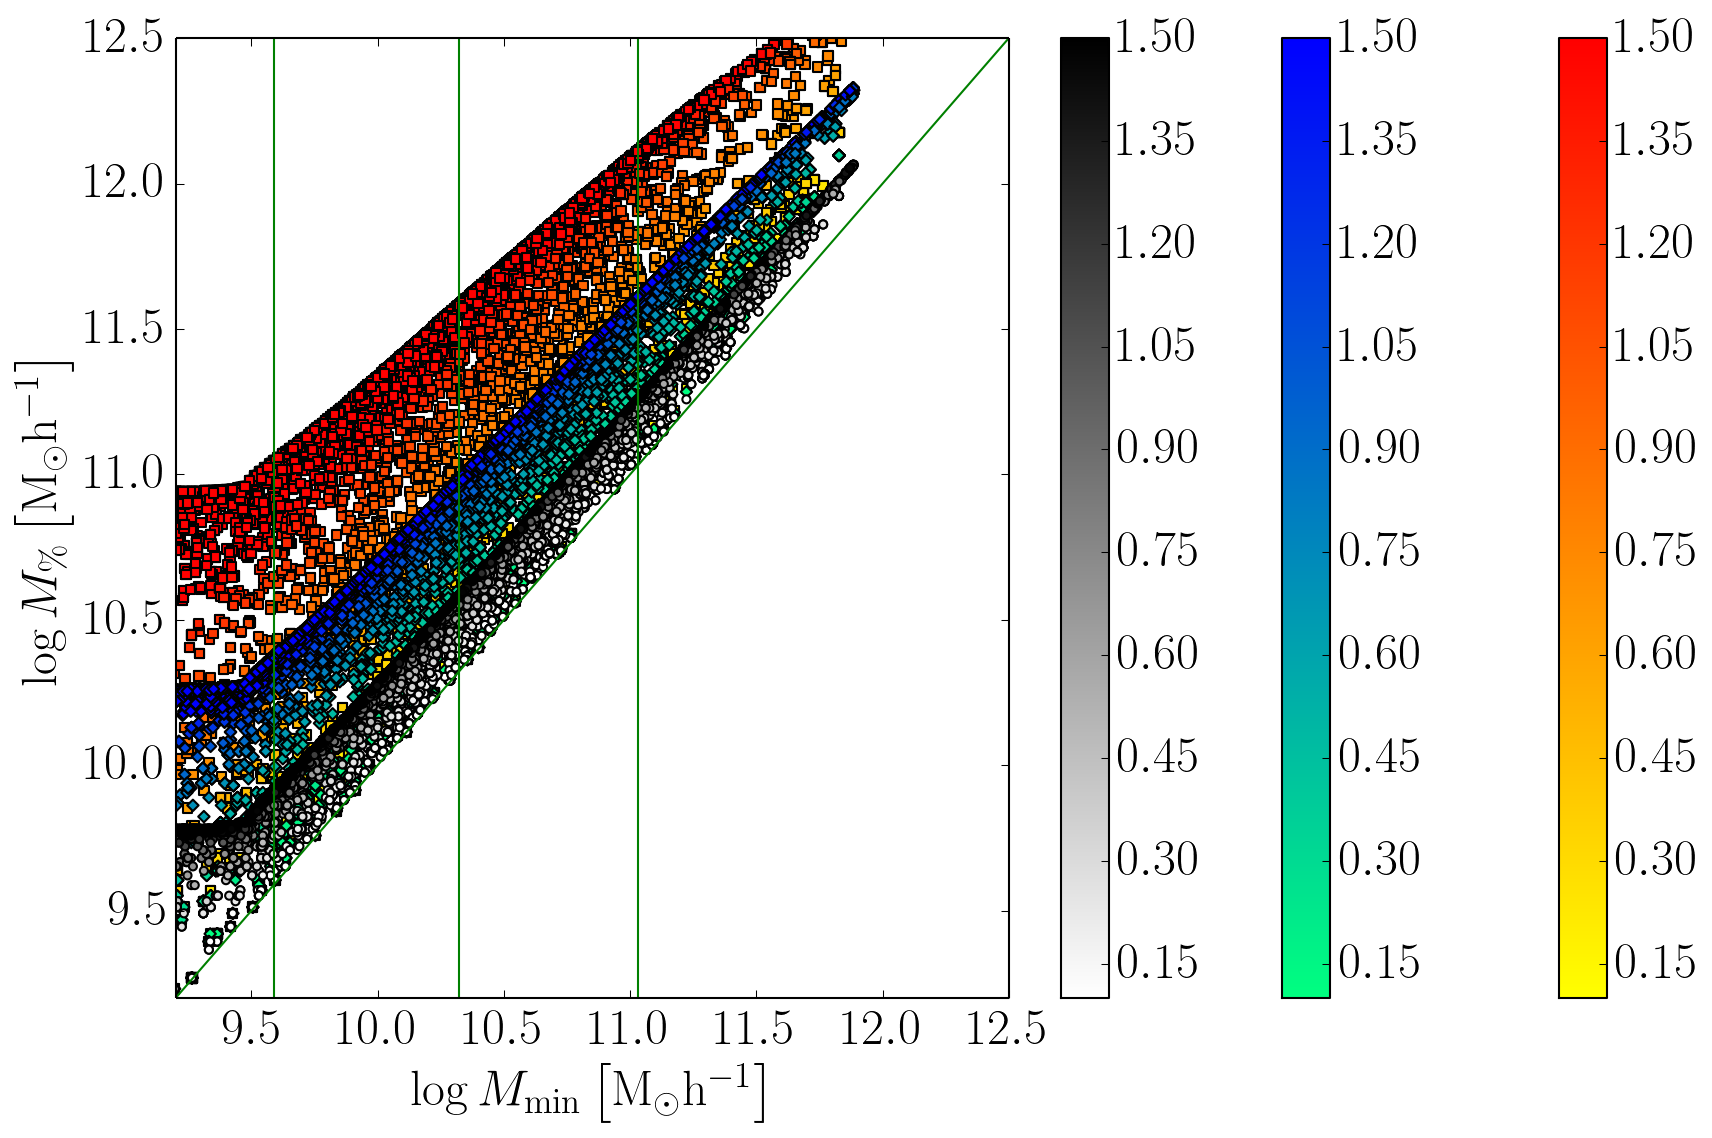
\includegraphics[width=0.47\textwidth]{mmin_mmed_colordm.png}
\caption{ $\log M_{\rm min}$ vs $\log M_{\rm 50\%}$ (black), $\log
  M_{\rm 16\%}$-$\log M_{\rm 84\%}$ (blue) and  $\log M_{\rm
    2.5\%}$-$\log M_{\rm 97.5\%}$(red) for different values of $\log
  M_{\rm max}$. The points are color coded by $\Delta \log
  M\left[\rm{M_{\odot}h^{-1} ]}\right]$. The green line diagonal line
accounts for the 1:1 relation and the green vertical lines represent
the 16, 50 and 84 percentiles  of the posterior probability
distribution of \mmin.} 
\label{fig:mmed}
\end{figure}

\subsection{Halo mass distribution within models}

Previous  attempts to constrain the DMH mass of LAEs by means of the
ACF   present their result in terms of the median mass of LAEs that is
derived from the derived correlation length by means of
semi-analitical prescriptions
\citep[e.g.][]{Hayashino2004,Gawiser2007,Ouchi2010,Bielby16}. Instead,
in this work we directly compare the ACF of our simulated mock
catalogs with the observational ACF and present our results in terms
of a  minimum and maximum mass DMH hosting LAEs. It is therefore
necessary to connect our approach by computing the median mass of the
DMH in each of the models $\mathcal{M}$.  In   Fig. \ref{fig:mmed} we
show the 50 ($\log M_{50}$, black dots), the 84 ($\log M_{84}$,blue
diamonds) and 95 ($\log M_{95}$, red squares) percentiles of the LAE
halo mass as a function of \lmmin\ for each of the models that we run
in our MCMC simulation.  The points are color coded according to their
\dlm\ associated value. We can see that the median mass ($M_{50}$) and
$M_{84}$ are not very sensitive to  $\lmmax=\lmmin +\dlm$ specially
when $\dlm\gtrsim1.0$dex. We particularly found that
$\lmmin\lesssim\log M_{50}\lesssim\lmmin+0.2\rm{dex}$ and that
$\lmmin+0.1\rm{dex}\lesssim\log M_{50}\lesssim\lmmin+0.5\rm{dex}$
regardless of the value of \dlm. The latter is a consequence of the
very steepen distribution of the dark matter mass function  and is at
the same time the reason for the almost perfect one to one relation
between \mmin\ and \focc. However, it can also be seen in
Fig. \ref{fig:mmed} that $\log M_{84}$ is very sensitive to \lmmax
($\lmmin+0.2\rm{dex}\lesssim\log
M_{50}\lesssim\lmmin+1.5\rm{dex}$). Thereby, any differences in the
clustering strength of models sharing the same \mmin but different
\mmax should be mainly driven by the  $\sim16\%$ most massive  halos
of each model $\mathcal{M}$.  

In order to estimate the effect of most massive halos in
$ACF_{\mathcal{M}}$ in Fig. \ref{fig:corr} we show the computed
$ACF_{\mathcal{M}}$ of models with $\lmmin=0.5$ and different values
of $\dlm$. We can see that the clustering gets stronger for larger
values of \dlm. Nevertheless, due to the large impact of cosmic
variance at the volume of the current observations all the models  are
basically consistent within errors. The last result together with the
large Poissonian observational error in the ACF explain the current
difficulty to put tighter constrains in \lmmax\ in our model. 

 In Fig. \ref{fig:mmed} the green vertical lines represent  the 16, 50
 and 84 percentiles  of the posterior probability distribution of
 \mmin that we previously obtained. From this figure we find that the
 median dark matter halo mass is $\tilde{M}_{\mathrm h} =
 10^{10.6^{+0.7}_{-0.6}} $. 
This result is consistent with previous
 estimations of  the  median dark matter halo mass reported by
 \citet{Bielby16} ($\tilde{M}_{\mathrm h} = 10^{11.0\pm0.6}$),
 \citet{Gawiser07} ($\tilde{M}_{\mathrm h} = 10^{10.9\pm0.9}$) and
 \citet{Ouchi2010} ($\tilde{M}_{\mathrm h} =
 6.7^{+42.0}_{6.7}\times10^{10}$) using semi-analitical approaches.   


\begin{figure}

  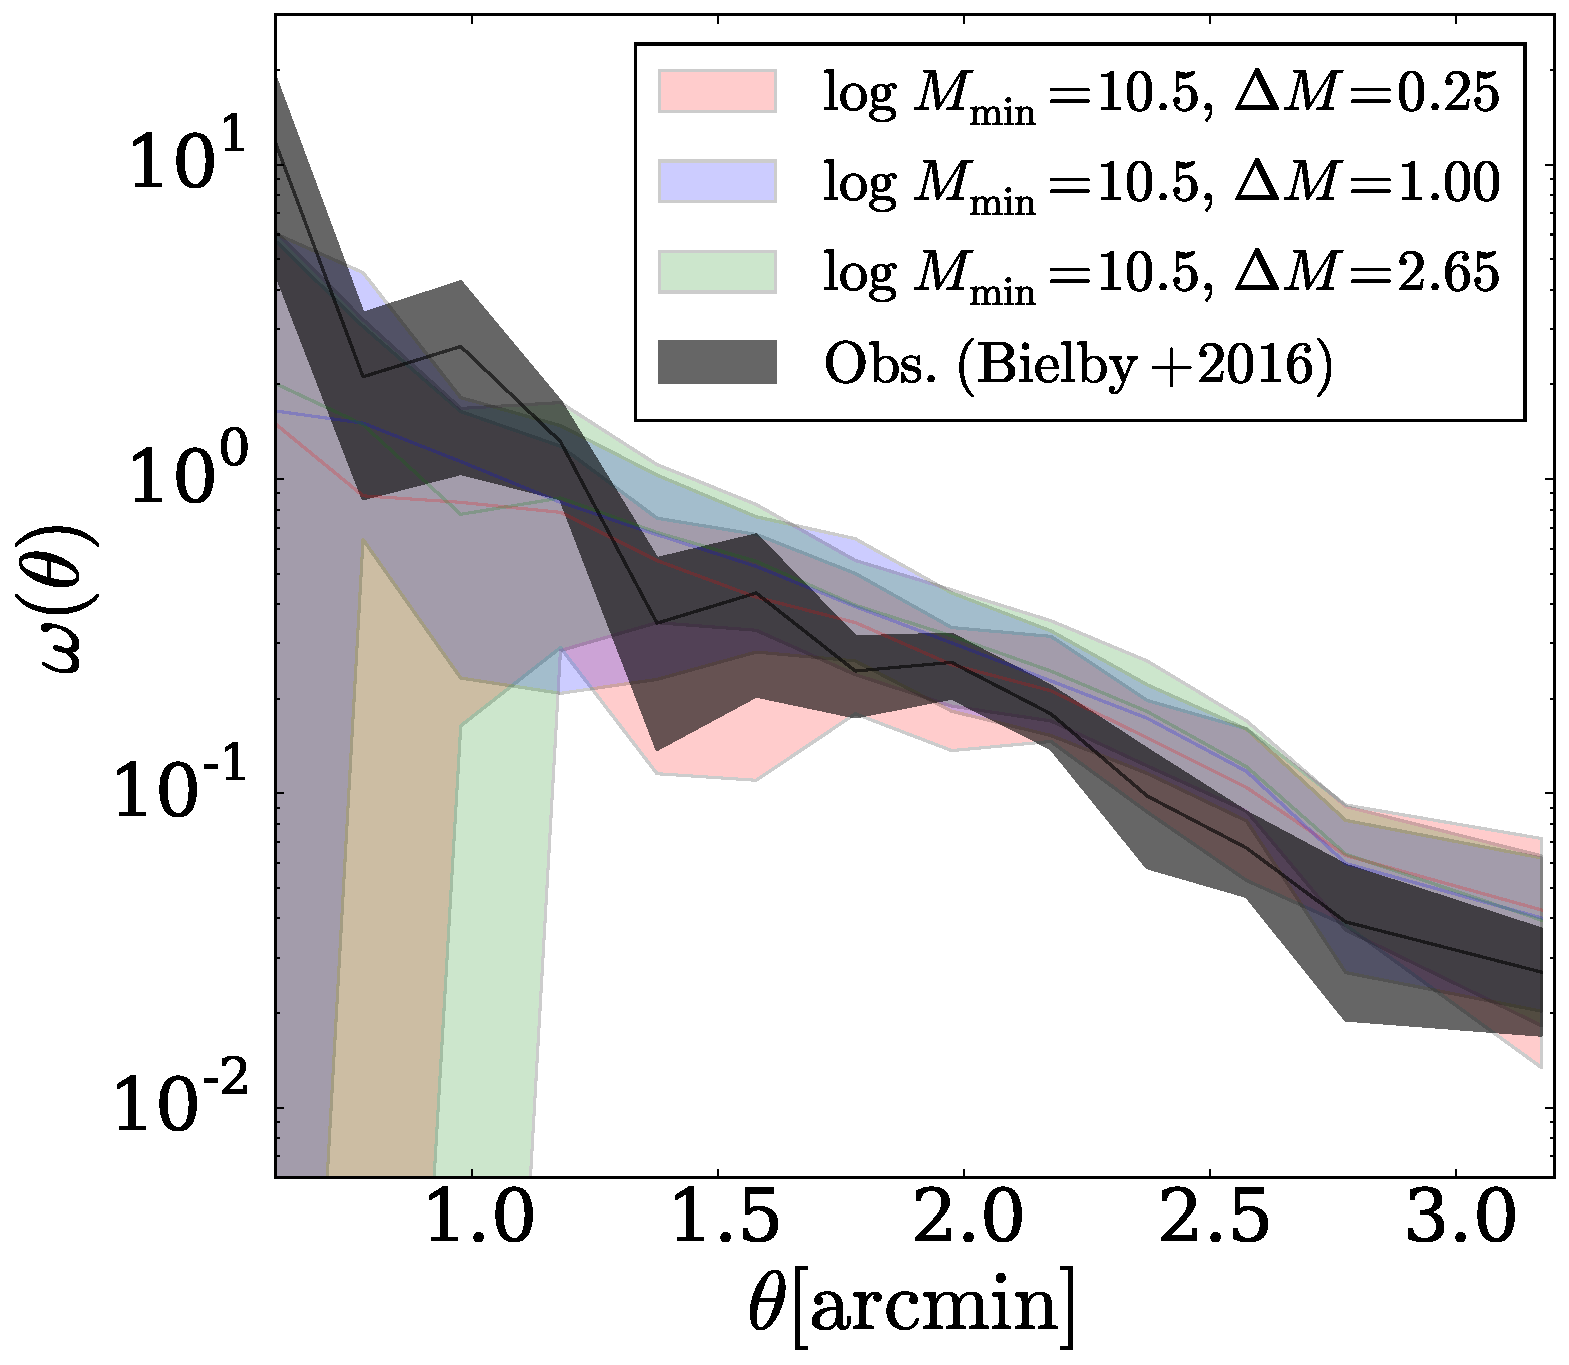
\includegraphics[width=0.47\textwidth]{fig5.pdf}
\caption{ Angular Correlation functions for $\log M_{\rm
    min}[\rm{M_{\odot}h^{-1}}]=10.5$ and different values of $\Delta
  M$.  
  The shaded region represents the 1-sigma deviation due to cosmic
  variance. Radical different models in $\Delta M$ are consistent with
  observations once cosmic variance is modelled in detail.}
\label{fig:corr}
\end{figure}



\subsection{Constraining Dark matter halos mass  with cosmic variance}
Fig. \ref{fig:cosmicv0}  shows the  halo number distribution (HND) in the  mock fields of the simulation for different models $\mathcal{M}$. By simple inspection one can infer an increase in the distribution with as \lmmin increase.  This trend is confirmed in Fig. \ref{fig:cosmicv}  where we plot the central 1-$\sigma$ (blue diamonds) and 2-$\sigma$  (red dots) widths  of the NDH as a function of \lmmin. We particularly found that when we consider survey fields of $\sim1{\rm deg^2}$, the central  1-$\sigma$ (2-$\sigma$) width of the HND increases monotonically from 0.05dex (0.10dex) when $\lmmin=9.5$ to 0.20dex (0.35dex) when $\lmmin=12.0$. The latter result opens the possibility to constrain the \lmmin (as well as the median mass) of LAEs by simply measure the width of the distribution of observed LAE along several observational fields mapping $\sim1{\rm deg^2}$ in area and the observational depth determined by the NB479 filter.



%*************************************************************************

\begin{figure}
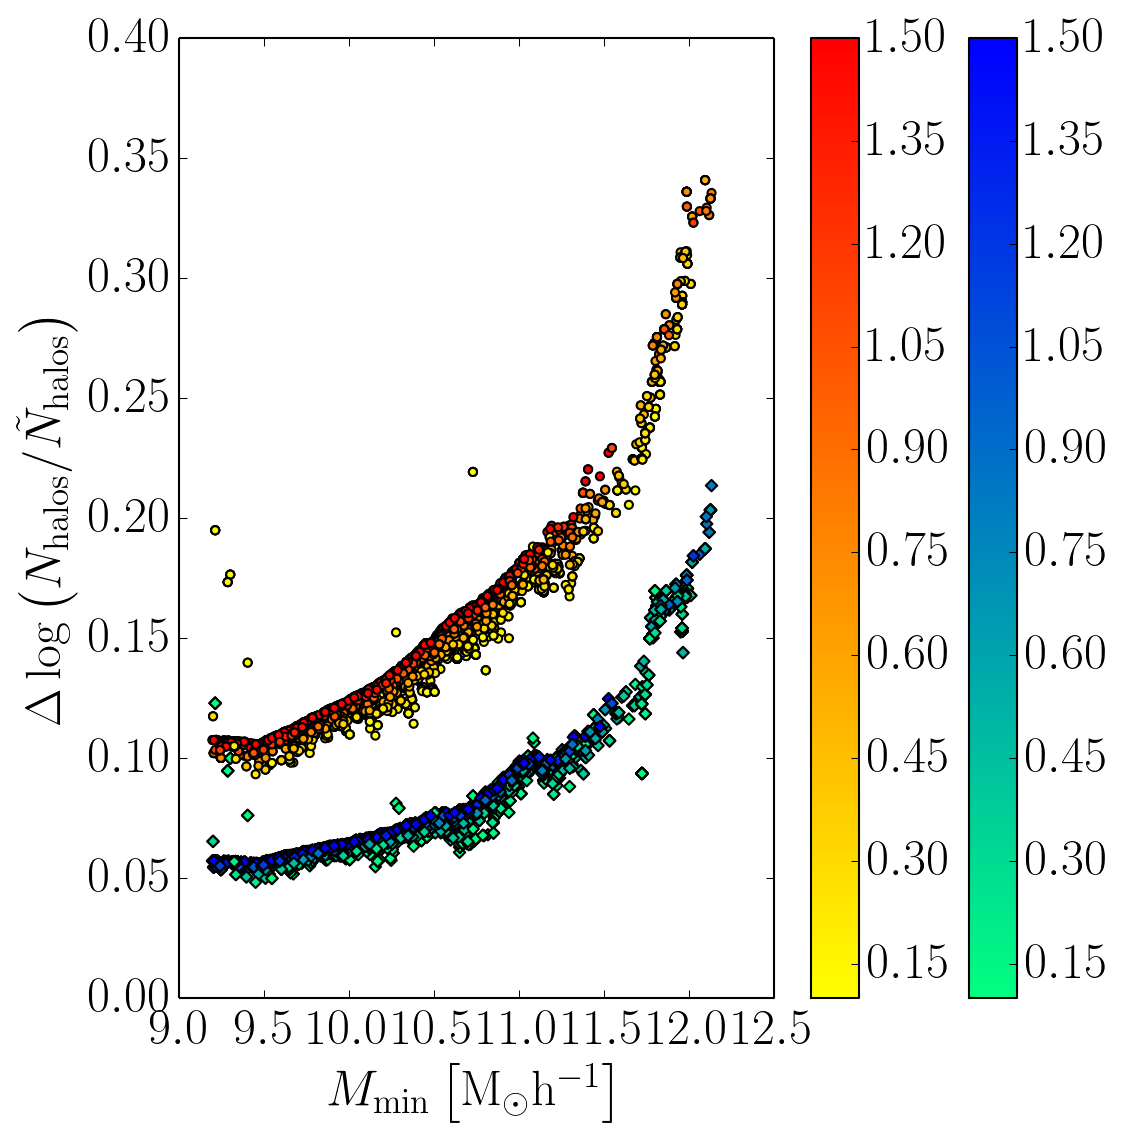
\includegraphics[width=0.46\textwidth, height=0.33\textwidth]{mmin_dfocc1.png}
\caption{Width of the halo number distribution over the 54 mock field of the simulation ($\Delta \log \left( N_{\mathrm halos}/\tilde{N}_{\mathrm halos}\right)$) of the central 68 (blue diamonds) and  95(red circles)  percentiles vs $M_{\rm min}$. Points are color coded according to their associated value of $\Delta M \equiv M_{\rm min}-M_{\rm min}$. The green line diagonal line accounts for the 1:1 relation and the green vertical lines represent  the 16, 50 and 84 percentiles  of the posterior probability distribution of \mmin.}
\label{fig:cosmicv}
\end{figure}


\section{Conclusions}

In this letter we studied the impact of cosmic variance and observational uncertainties in constraining the mass range and  occupation fraction of dark matter halos hosting  LAEs.  
To this end, we used the BolshoiP N-body simulation to construct  27 mock fields  with the same typical size  of observed fields at  $z=3.1$ ($\sim 1 {\rm deg^2}$).  
In our model a dark matter halo with mass in the range $M_{\rm min}<M_{\mathrm h}<M_{\rm   max}$ can only host one detectable LAE at most. 
We explored the parameter space determined by \mmin\ and \mmax\ using Monte Carlo Markov-Chain minimization to match the observed  ACF and mean number density of LAEs. 

Our analysis allowed us to put weak constraints on $M_{\rm min}$, $M_{\rm max}$ and $f_{\rm occ}$ where $10^{9.7}\hMsun\leq \log M_{\rm min}\leq 10^{11.2}\hMsun$, $10^{10.9}\hMsun\leq \log M_{\rm max}\leq 10^{13.0}\hMsun$ and $0.02\hMsun\leq f_{\rm occ}\leq 0.5$, spanning three orders of magnitude in halo mass.
Previous works\citep{Hayashino2004, Gawiser07,Ouchi2008,Bielby16} have found typical masses within somehow narrower mass ranges ($\sim 10^{10.5}$-$10^{12}$).  
The main reason for our weaker constraints and large discrepancies with previous works resides in the cosmic variance on the typical field size in observations. 
A thorough exploration of cosmic variance impact as we present in this letter had not been presented so far in the literature.

Our analysis also allowed us to draw three results that can be used to put tighter constraints on $M_{\rm min}$, $M_{\rm max}$ and $f_{\rm occ}$ once upcoming large LAE surveys, as the HETDEX project \citep{Hetdex2011} and the HSC ultra deep survey, are available :
\begin{enumerate}
\item $f_{\rm occ}$ and the median mass of LAEs are almost uniquely determined by $M_{\rm min}$ regardless of $M_{\rm max}$. \item measuring the width of the LAE number distribution function obtained over several fields of $\approx 1$ deg$^2$ one will be able to tightly constrain  $M_{\rm min}$, $M_{\rm med}$ and $f_{\rm occ}$ up to a factor of  2. 
\item  $M_{\rm max}$ drives the ACF strength at short angular distances ($<1\,\rm arcmin$), therefore precise measurements of the ACF at such scales are crucial to accurately determine \mmax.
\end{enumerate}



\section*{Acknowledgments} 

JM acknowledges ``CONICYT-PCHA/doctorado Nacional para extranjeros/2013-63130316'' for their PhD scholarship support. 


\bibliographystyle{apj}
\bibliography{references.bib}

\end{document}
